%% Template for SDP report, adapted from mlp_cw2_template, 2018. 

%% Based on  LaTeX template for ICML 2017 - example_paper.tex at 
%%  https://2017.icml.cc/Conferences/2017/StyleAuthorInstructions
\usepackage{xcolor}
\documentclass{article}
\usepackage[T1]{fontenc}
\usepackage{amssymb,amsmath}
\usepackage{txfonts}
\usepackage{microtype}
\usepackage{xspace}
\xspaceaddexceptions{\%}
\usepackage{subcaption}
% Lists with less spacing between items
\usepackage{paralist}
\usepackage{tabularx}
\usepackage[normalem]{ulem}
% For figures
\usepackage{graphicx}
\usepackage{subfig} 

% For citations
\usepackage{natbib}

% For algorithms
\usepackage{algorithm}
\usepackage{algorithmic}

% the hyperref package is used to produce hyperlinks in the
% resulting PDF.  If this breaks your system, please commend out the
% following usepackage line and replace \usepackage{mlp2017} with
% \usepackage[nohyperref]{mlp2017} below.
\usepackage{hyperref}
\usepackage{url}
\urlstyle{same}

% Packages hyperref and algorithmic misbehave sometimes.  We can fix
% this with the following command.
\newcommand{\theHalgorithm}{\arabic{algorithm}}


% Set up MLP coursework style (based on ICML style)
\usepackage{mlp2018}
\mlptitlerunning{SDP Demo \demoNumber  Group (\groupNumber)}
\bibliographystyle{icml2017}


\DeclareMathOperator{\softmax}{softmax}
\DeclareMathOperator{\sigmoid}{sigmoid}
\DeclareMathOperator{\sgn}{sgn}
\DeclareMathOperator{\relu}{relu}
\DeclareMathOperator{\lrelu}{lrelu}
\DeclareMathOperator{\elu}{elu}
\DeclareMathOperator{\selu}{selu}
\DeclareMathOperator{\maxout}{maxout}







%% You probably do not need to change anything above this comment

%% REPLACE the details in the following commands with your details
\setGroupNumber{4}
\setGroupName{Sprout.ed}
\setProductName{Sprout.ed}
\setDemoNumber{2}
\setLogoFileName{figs/sprouted_logo.png}

\definecolor{mygray}{RGB}{102, 102, 153}
\definecolor{mybrown}{RGB}{102, 51, 0}



\begin{document} 

\makeSDPTitle{Demo}

% Previous MLP Style Title Layout working. 
% \twocolumn[
    % \mlptitle{\productName: SDP Demo \demoNumber}
    % \centerline{Group \groupNumber: \groupName}
% ]

\begin{abstract} 

Sprout.ed is a 3-axis planting and watering system designed for office space well being, with a web app allowing for an overview and management of the currently growing plants. 

Sprout.ed has taken root since the last demo, introducing a head with vertical and horizontal movement, meaning all 3 axes of movement are now utilised. On startup, the system now calibrates to the size of its frame through stopper switches and constructs a 2D grid system within this size. Additionally the overall construction has been made more robust and a design for the planting drillbit was formalised. In terms of the web app, functionality is now divided across different pages on the web app drawing from our Figma prototype, with real-time sensor data displayed via graphs on the admin page as well as an on demand webcam photo on the landing page.

\end{abstract} 

\section{Project plan update}
\subsection{Milestone 2 goal updates}
We were organized into three sub-teams again working towards this milestone, and all sub-teams achieved 100\% of the goals. The teams and their milestones for this demo are described below.
\subsubsection{\textbf{Mechanical Team - Anukrat, Rokas, Yichao}}
\vspace{3mm}
\begin{itemize}
    \vspace{-3mm}
    \setlength{\itemsep}{0pt}%
    \setlength{\parskip}{0pt}
    \item (Achieved) Horizontally movable head on top of the gantry
    \item (Achieved) Vertically movable arm that can move vertically in place
\end{itemize}
\textbf{Mechanical team} outlined a design for the movable head, arm and the plant bed, then decomposed the task for members to work in parallel. Rokas built the first iteration of the movable head and arm, and later assembled the custom-wood platform for sprout.ed. Yichao reinforced the stability and strength of the movable head. Anukrat designed the wooden base and the frame. Rokas and Yichao then worked to add sensors reliably to the robot, while Anukrat managed the increasing number of cables on the robot. In the end, they also designed the drillbit for planting the seeds (which was for Milestone 3).
\subsubsection{\textbf{Electrical Team - Alan, Shreyas, Serena, Terry}}
\vspace{3mm}

\begin{itemize}
    \vspace{-3mm}
    \setlength{\itemsep}{0pt}%
    \setlength{\parskip}{0pt}
    \item (Achieved) Motors set up to move in all 3 axes
    \item (Achieved) Set up a 2D Grid system
    \item (Achieved) Trigger movement of head based on low soil moisture levels
\end{itemize}

\textbf{Electrical team} decided to divide the team in to two groups. Alan and Shreyas worked on moving the motors along all 3 axes and setting up a 2D Grid System, while Terry and Serena focused on setting up additional moisture and temperature/humidity sensors. However, we later decided to replace these sensors with one moisture sensor on the arm. The 2D Grid system now allows the user to input a coordinate like (2,3) into the web app to move the head to that position. Terry and Serena also worked on an extension for the project: implementing communication to a webcam to monitor plants.
\subsubsection{\textbf{Webapp Team -  Balraj, Dima, Sonia}}
\vspace{3mm}
\begin{itemize}
    \vspace{-3mm}
    \setlength{\itemsep}{0pt}%
    \setlength{\parskip}{0pt}
    \item (Achieved) Display updated sensor data at a time interval and graphs of sensor data history
    \item (Achieved) Implement basic UI
    \item (Achieved) Implement data structure to store plant data and allow addition and removal of plants
\end{itemize}
\textbf{Web App team} planned out what data needs to be stored in the app and discussed what technologies to use, debating the benefits and disadvantages of each. After choosing to use JSON rather than a database to store the data and choosing React as a front-end framework for our web app, we split the tasks between us. Sonia implemented an initial basic UI for the web app, using HTML, CSS and Javascript, then investigated how to best use React in our app. Balraj implemented a data structure to store plant data in a file and display it on the web app using the flask web server, and then the functionality of adding and removing plants to and from the data structure from the web app. Dima implemented charts which update in real time, displaying the output of the connected sensors and explored options for scheduling tasks on the frontend and backend. Dima and Sonia then worked with the Electrical team on the extension to display a photo from the webcam on demand. We decided to use only one Github repository, rather than one for backend and one for frontend, as all the code is interconnected. Sonia streamlined the method of getting updated code on and off the Raspberry Pi using git.

\subsection{Milestone 3 Goal Modifications}
Having reached Demo 2 and achieved our Milestone 2 goals, we have now considered the next steps and made the following clarifications to the goals for Milestone 3.

\textbf{Mechanical Team:}
\begin{itemize}
    \vspace{-3mm}
    \setlength\itemsep{-0.6em}
    \item Digging/drilling utensil - designing and manufacturing a part capable of piercing soil that would be attached to a motor at the end of the vertical arm. Digging/softening of soil would be achieved by rotating the utensil.
    \item Watering system - water being represented by light (e.g. LED strip) with realistic positioning of the hose that would be used with a water tank.
    \item Seed deployment system - consisting of an air pump with a specialized head for picking up and releasing seeds, as well as a system of containers for different types of seed.
    \vspace{-3mm}
\end{itemize}
\textbf{Electrical Team:}
\vspace{-1mm}
\begin{itemize}
    \vspace{-3mm}
    \setlength\itemsep{-0.4em}
    \item Automated watering - combining sensor readings along with plant requirements to decide optimal watering times.
    \item Digging/drilling related movements - precise motor rotations to pierce the soil, which will be tested by a button click on the webapp 
    \vspace{-3mm}
\end{itemize}

\textbf{Web App team}:
\vspace{-1mm}
\begin{itemize}
    \vspace{-3mm}
    \setlength{\itemsep}{0pt}
    \setlength{\parskip}{0pt}
    \setlength{\topsep}{0pt}
    \item Action history and error log - the admin page will display timestamped actions taken on the web app, such as 'Image taken at 03:15:00' or 'Head moved to position (3,4) at 4:45:12'.
    \item Implement plant dashboard - the dashboard will display the current plants, clicking on a plant will bring up information about it and an option to remove it, and clicking on an empty spot will allow a plant to be added
    \item Implement watering controls - will be able to select individual plants to water as part of the admin plant dashboard
\end{itemize}

\section{Technical details}
\subsection{Mechanical}

The duties of mechanical team for the second milestone can be split into two tasks: constructing the gantry head and arm, and the wooden base. 

The gantry head used a very similar design to the one seen at the base of the gantry. The one difference is a lack of wheels, and the use of medium-EV3 motors, which is justified with the fact that the head needs to support significantly less weight than the gantry to warrant using limited space on the head for friction reducing measures. 

\begin{figure}[h]
\begin{center}

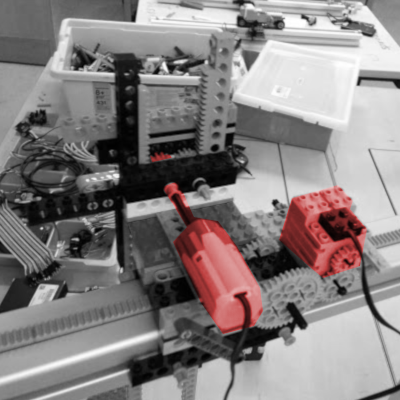
\includegraphics[width=0.32\linewidth]{figs-demo2/motors1.png}
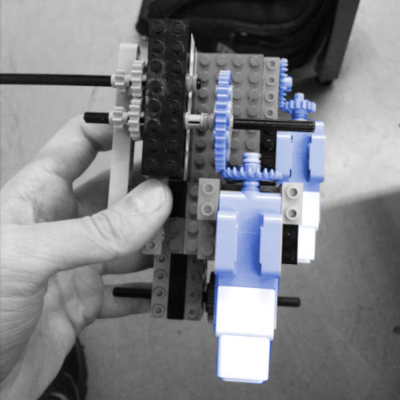
\includegraphics[width=0.32\linewidth]{figs-demo2/motors2alt.png}
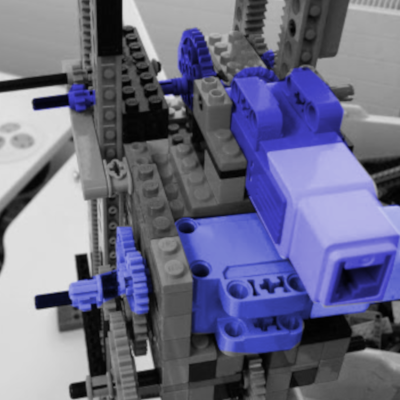
\includegraphics[width=0.32\linewidth]{figs-demo2/motors3alt.png}

\caption{from left to right: iteration 1,2 and 3 of motor arrangement.}
\label{fig:motors}
\end{center}
\vskip -4mm
\end{figure} 

The head involved several iterations, mainly related to the vertically-moving arm attached to it. The most troublesome part was fitting two motors on it - one for moving the head horizontally, one for moving the arm vertically. To conserve space, smaller motors were considered, but were later replaced with EV3 to simplify and unify the implementation for motors responsible for spatial movement. The mechanism for vertical movement stayed the same from the first iteration, but was doubled up to provide greater stability and more space for the tools that will be attached to the arm in the future (see Figure \ref{fig:arms}). This required repositioning of the motors (see Figure \ref{fig:motors}).

\begin{figure}[h]
\centerline{
\begin{subfigure}[b]{0.4\columnwidth}
    \centerline{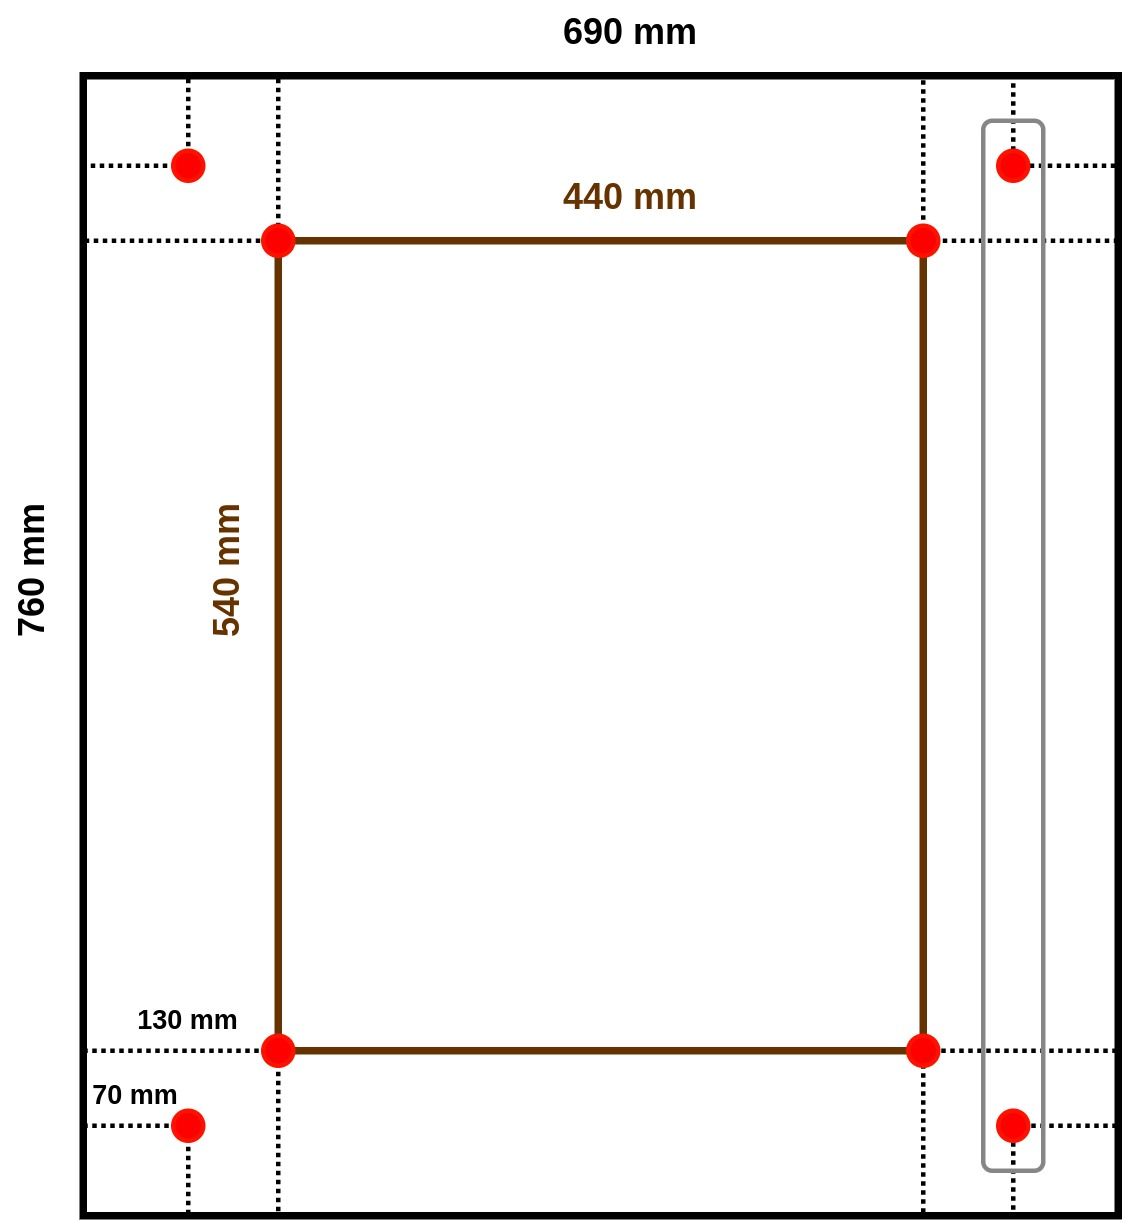
\includegraphics[width=\linewidth]{figs-demo2/frame.jpg}}
    \subcaption{}
    \label{fig:bed}
\end{subfigure}
\begin{subfigure}[b]{0.35\columnwidth}
    \centerline{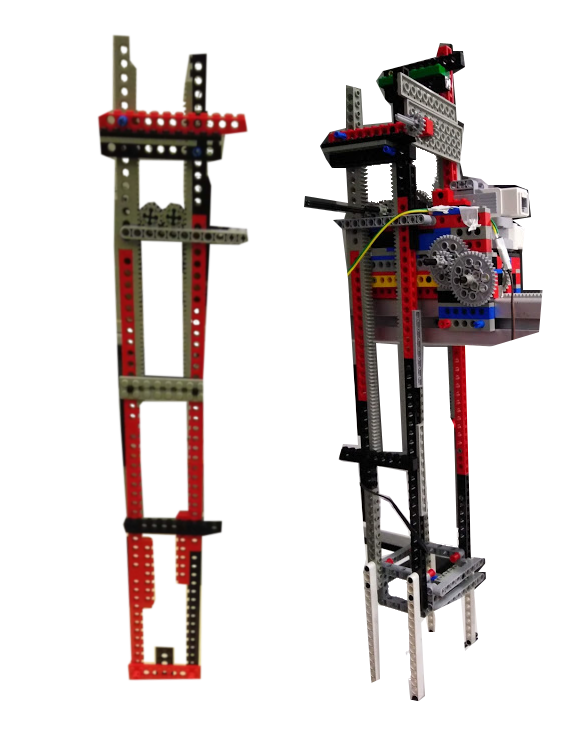
\includegraphics[width=\linewidth]{figs-demo2/p.png}}
    \subcaption{}
    \label{fig:arms}
\end{subfigure}
}

\caption{(a) The diagram of the base. \textcolor{red}{Red} circles mark the holes for drilling, the walls of the plant bed are colored \textcolor{mybrown}{brown}. \textcolor{mygray}{Gray} rectangle shows how the gantry frame would fit on the base.
(b) left - initial arm design, right - doubled-up and reinforced arm design}

\vskip -5mm
\end{figure}


The base was ordered to be cut by the technician team. The mechanical team measured the optimal distance between the frame of the gantry and the plant bed and sketched a diagram of it for the order. The measurements of the base can be seen in Figure \ref{fig:bed}.

\subsection{Electrical Team}

\subsubsection{Moving Motors in all 3 axes}

This task was fairly straightforward as the EV3 brick supports the Large and Small motors and requires only a few lines of Python code to get the motors moving. The Mechanical team had set up the motors in place on time which helped us complete this milestone very early.

\subsubsection{2D Grid Set-up}
Alan and Shreyas then worked on setting up the 2D System which means splitting the plant bed into a multiple-coordinate system to allow the head to go over every coordinate on the plant bed. To test this easily we decided the best way would be to have the user input a coordinate into the web app which is then forwarded to the EV3 which moves the motors to the desired coordinate.

Before starting to implement this, we realised that the EV3 needs to know the length of the base rail and gantry so that it can validate the commands it receives i.e. reject a value that would correspond to a point outside the scope of the plant bed. To do this, we need to calculate the number of steps (technically, the pulses of the rotary encoder) required to move the motors from one end of the rail to the other. We achieved this by using touch sensors on both ends of the rail. On booting, the base rail motors and gantry motors simultaneously move to the furthest end and then calculate the number of steps it takes to traverse the rails and gantry. This gives us the required lengths. 
We initially planned to use ultrasonic sensors to know the location of the motors but after speaking to the SDP technical staff, we were told that the number of rotations along with touch sensors at each end would be sufficient. We researched more and decided to implement this. 

To split the grid into coordinates, we decided that 2.5cm by 2.5cm on the base rails and gantry is a suitable minimum distance between points on each axis for our use case of working with indoor plants. We then calculated the number of steps the motor needs to travel this distance by returning the “position” value of the rotary encoder. This was 1000 for the large motors and 750 for the smaller ones. Moving to a coordinate (2,3) now meant moving the large motors (base rail) by $2*1000 = 2000$ pulses and the small motors (gantry) by $3*750 = 2250$ pulses.

Once we achieved movement to any desired coordinate, we were able to set up endpoints on the web app which communicate through the TCP server and motors to direct the head to user-supplied co-ordinates. 

\subsubsection{Triggering Watering Across 2D Grid by Sensor Readings}
In order to achieve this goal, Terry and Serena first considered planting multiple moisture sensors into the soil, giving constant readings to the Pi which would monitor the data and command the EV3 to move to a certain coordinate based on where the sensor is. However, this would have required many moisture and humidity/temperature sensors which is expensive and would put undue pressure on the Pi. Thus they decided to attach one moisture sensor to the arm, and Alan and Shreyas designed a new script which would run every 15/20 minutes. The script would command the arm to move across the diagonals and the center, measuring the moisture level at the coordinate, comparing it to the threshold, and then either moving on to the next coordinate or watering at that coordinate (as represented by the LED lighting up).

\subsubsection{Sensor Reliability}

Since demo 1, we decided to take multiple readings to avoid discrepancies in moisture measurements, so now we detect moisture levels three times per reading. Additionally, we added a function which determines moisture thresholds according to different plants. Sensors are bound to the arm to test the soil moisture levels when extended.

\subsubsection{Camera Set-up}
We decided to set a webcam on the gantry to capture an image and display it on the website by using pygame, which includes an accessible graphics library. We initially decided to use a picamera but later decided to use a webcam as it has a higher resolution and is less restrictive on construction due to its longer cable.

\subsection{Web Application Team}
\subsubsection{Data Implementation}
We have decided to use JSON to store data in our web app, data such as the details of currently planted plants, and historical sensor readings. We considered a few options for storing data, including different database implementation such as SQL or NoSQL. Through research and discussions we came to a conclusion that these would be ideal if we were dealing with thousands of readings or needed relationships between different records, but for this project we felt a database would add needless complexity and thought a lightweight solution would be preferred. JSON is easily interpretable, straightforward to read/write to and simple to work with while still meeting our needs for this project. Since our emphasis is on data representation we concluded that JSON was the best solution.

\subsubsection{User Interface}

We decided to use the front-end framework \href{https://reactjs.org/}{React} in our web app. Frameworks like React offer a host of advantages for web app development, they allow for the easy reuse of components, offer already existing templates (meaning we don’t have to waste time re-inventing the wheel), and encourage separating the frontend and backend so that components can be updated without reloading the whole page. Multiple other frameworks such as \href{https://angularjs.org/}{AngularJS} and \href{https://vuejs.org/}{Vue} are available, but after research we felt there was not much differentiation between them for our use case but the comprehensive documentation provided by React gave us reason to choose it.

\subsubsection{Usability Considerations}
In order to ensure the right decisions for usability of our user interface, we have decided to use the \href{https://material.io/resources/color/#!/?view.left=0&view.right=0}{Material Design Color Tool} to choose the best colours for our design. This allows us to select colours which complement each other and also gives us accessibility metrics along with guidelines to follow with respect to text size and text/background colour pairing for visibility. The information for our intended colour scheme can be found at \href{https://material.io/resources/color/#!/?view.left=1&view.right=0&primary.color=E8F5E9&secondary.color=F5F5F5&secondary.text.color=212121&primary.text.color=2E7D32}{this link}. All chosen colours can be seen in Figure \ref{fig:colourscheme}.

\begin{figure}[h]
\begin{center}
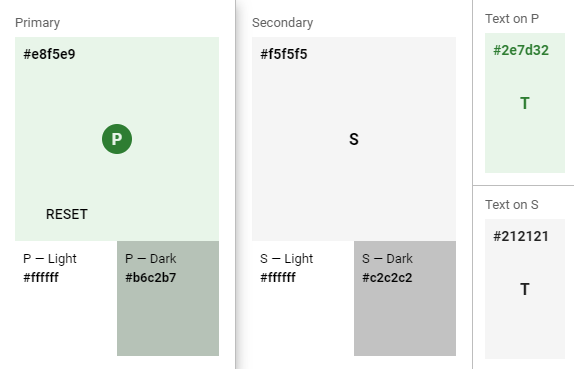
\includegraphics[width=\columnwidth]{figs-demo2/colourscheme.png}
\caption{The chosen colour scheme.}
\label{fig:colourscheme}
\end{center}
\vskip -5mm
\end{figure}

\subsubsection{Scheduling}
Python offers a few built in methods for scheduling (namely time.sleep and threading.Timer), there are also packages available such as \href{https://docs.celeryproject.org/en/stable/getting-started/introduction.html}{Celery}, which provides asynchronous job queuing and scheduling. Celery is the de facto solution but proved to be overkill for our needs while many of the inbuilt threading or timer functionality was clunky with regards to concurrent processes or \href{https://stackoverflow.com/questions/25676835/signal-handling-in-multi-threaded-python}{prone to errors on shutdown}. We found a lightweight package called Timeloop which provides function decorators for running multiple periodic tasks.


\section{Evaluation}

\subsection{Gear Efficiency}

The focus of any movement in the robot is precision over speed, with no functionality of the system adhering to strict time constraints. Thus, our aim when transferring force between gears is to maximise it in exchange of losing travel distance.

To the same purpose, friction was considered. Due to the difficulty of finding the correct friction coefficients for particular materials (LEGO brand ABS plastic and aluminum), the calculations have wide margins of error. Several similar materials were chosen and compared to arrive at a dynamic friction coefficient of \(\mu = 0.5\) between ABS and aluminium, \( \mu = 0.6 \) between ABS and ABS, and \( c_{rr} = 0.005 \) between the wheels and aluminium at the base. \cite{friction1}, \cite{friction2}

The weights of parts were also estimated. The weight of aluminum parts was estimated by taking the measurements of the gantry, calculating its volume and multiplying by the standard density of aluminium. The weight of the LEGO was estimated from the weight of one brick \cite{legoweight}.

Based on the torque of the EV3 motors \cite{motors2}, final torque of the gears (their diameters found here: \cite{gears}) in contact with the rails was calculated \cite{calc}, as well as the tangential force, and from that finally the friction, giving these results:
\vspace{-3mm}
\begin{figure}[h]
\begin{subfigure}[b]{0.25\columnwidth}
\centerline{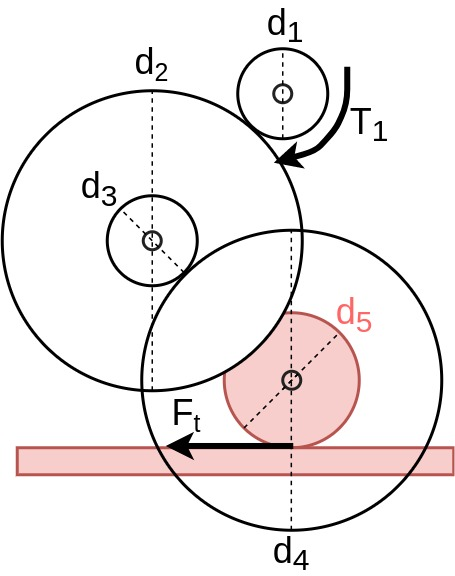
\includegraphics[width=\linewidth]{figs-demo2/HEADGEARS.jpg}}
\caption{}
\end{subfigure}
\begin{subfigure}[b]{0.25\columnwidth}
\centerline{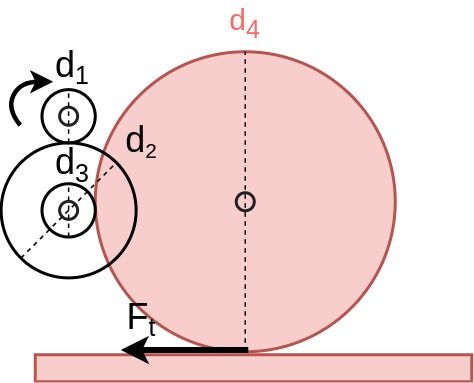
\includegraphics[width=\linewidth]{figs-demo2/BASEGEARS.jpg}}
\caption{}
\centering
\end{subfigure} 
\centering
\begin{subfigure}[b]{0.48\columnwidth}
\centerline{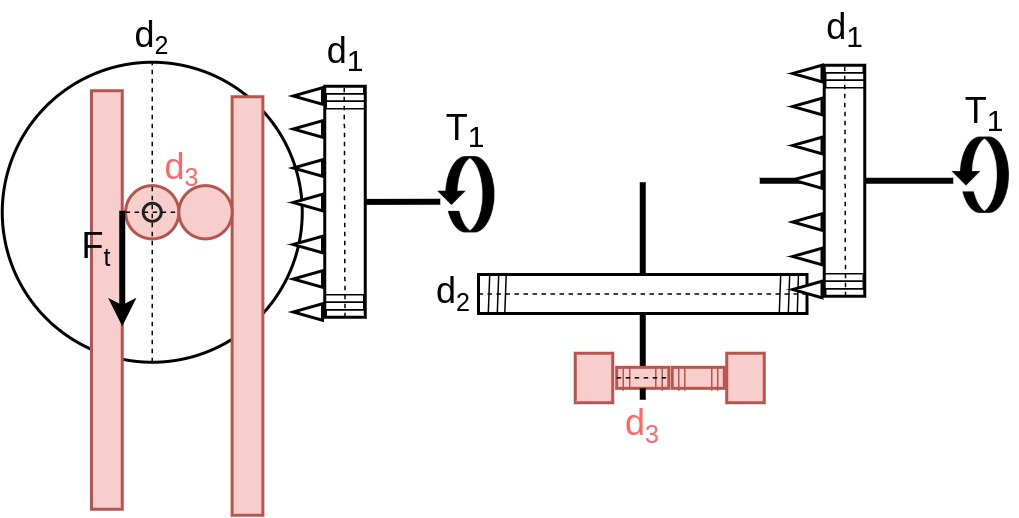
\includegraphics[width=\linewidth]{figs-demo2/ARMGEARS.jpg}}
\caption{}
\end{subfigure}
\end{figure}
\vspace{-3mm}

\begin{tabular}{|p{1.2cm}|p{1.1cm}|p{1.5cm}|p{1.5cm}|p{0.7cm}|}
\hline
            & Torque Ratio  & Moving Force, N & Friction Force, N & Mass, kg \\
\hline
Head (a)               & 6.104         & 39.06           & 0.171        & 0.45   \\
\hline
Arm (b)                & 2.471         & 43.92          & 0.059        & 0.1   \\
\hline
Base (c)               & 1.763         & 167.90         & 0.222        & 4.52 \\
\hline
\end{tabular}


Based on these results we can make a few observations:
(1) Use of wheels and replacing sliding friction with rolling resistance significantly reduced friction on base movement. \\
(2) the torque ratios in all cases show that the initial torque of the motor is increased by the arrangement of the gears. \\
(3) the highest force achieved corresponds to the heaviest object being moved, while lighter parts such as head and arm have significantly lower forces acting upon them. \vspace{0.5mm}

As we are using few motors, the calculation of gear friction with estimated coefficients would yield negligible results and as such was seen as trivial for now.

\subsection{Movement Accuracy}

Once we created the 2D grid system, it was crucial to test the accuracy of the motor movements. This was done by attaching a marker to the end of the arm to mark its position with dots. We wrote code to iteratively move the head to each grid point, move the arm downward to mark a point, lift the arm and continue.  After 20 iterations we found that the markings at each grid point varied by at most 1mm. We could see that this was due to instability of the arm and not due to the motors. The mechanical team was informed and they will work on stabilising the arm. 

At the same time, we marked the motor stop points on each of the rails for each iteration. The motor accuracy is 100\% (within the error bound of \( \pm 0.5 mm\)) as the points on the rails always overlapped perfectly with the previous iterations. 
\section{Budget}\label{budget_account}

{\footnotesize
\begin{tabular}{ |p{2.8cm}|p{1.6cm}|p{1cm}|p{0.9cm}|  }
\hline


\hline
\textbf{Name}& \textbf{Unit Price} &\textbf{Quantity} & \textbf{Price} \\
\hline
LEGO & £15.00/kg &1.00 kg &£15.00 \\
\hline
3D printing [4 parts] & 5 p/g   & 295.00 g & £14.75 \\
\hline
RSPro Aluminium struts &£41.00/3.00 m & 2.30 m & £31.46 \\
\hline
Angle joints for RSPro struts    &£5.00 each & 2 & £10.00 \\
\hline
Wooden Base & £8 for 2.43 x 1.21 m & 0.69 x 0.79 m & £1.48\\
\hline
Coriander seeds & 5.90/kg & £0.10 kg &£0.59   \\
\hline
Wooden struts & £2.50/m & 1.00 m & £2.50 \\
\hline
Grove Hat & £7.95& 1& £7.95 \\
\hline
Grove Moisture Sensor & £3.56 & 1 &£3.56 \\
\hline
DHT11 temp, Humidity Sensor & £3.59 & 1 & £3.59 \\
\hline
Raspberry Pi 3 & £23.00 & 1 & £23.00 \\
\hline
LEGO EV3 & £202.00 & 1 & £202.00 \\
\hline
LEGO EV3 Large Motors & £25.00 & 2 & £50.00 \\
\hline
LEGO EV3 Medium Motors & £25.79 & 2 & £51.58\\
\hline
Wood Board  & £8 for 2.43 x 1.21 m & 2 (0.10 x 0.54 m each) & £0.29\\
\hline
Wood Board & £8 for 2.43 x 1.21 m & 2 (0.10 x 0.44 m each) & £0.24 \\
\hline
Touch Sensor & £16.00 &4 & £64.00 \\
\hline
Technician Time & - &2 hours & - \\
\hline
Logitech Camera &£27.00  &1 & £27.00 \\
\hline
Miscellaneous (eg. Screws, Bolts, Tape) & - & - & £5.00 \\
\hline
\textbf{TOTAL}  & - & - & £513.99 \\
\hline
\end{tabular}
}



%% Include any references in a bibliography

\bibliography{demo2-refs}

\end{document} 



